% =============================================================================
%  avance_socioformador_tecnico.tex - presentacion breve de avance (issue #64)
%  VERSION TECNICA: mismas cifras que avance_socioformador.tex, redaccion
%  con terminologia estadistica (razones de momios, homocedasticidad,
%  prueba de DeLong, etc.), para una audiencia con ese conocimiento previo.
%
%  NO es la presentacion final de entrega: es un medio para mostrarle al
%  socioformador el avance tras el cambio de objetivo y recibir
%  retroalimentacion. Compila independiente de reports/ (misma carpeta de
%  figuras, via \graphicspath, para no duplicar archivos).
%
%  Fuente de las cifras: reports/secciones/objetivo_tecnicas.tex,
%  reports/secciones/pca.tex y reports/secciones/regresion_logistica.tex.
%
%  Compilar desde esta carpeta:   latexmk -jobname=avance_socioformador_tecnico avance_socioformador_tecnico.tex
% =============================================================================

\documentclass{beamer}

\usetheme{Madrid}
\usecolortheme{default}

\usepackage[T1]{fontenc}
\usepackage[utf8]{inputenc}
% Igual que reports/main.tex: es-nodecimaldot evita que babel convierta
% los puntos decimales en comas dentro de modo matematico.
\def\spanishoptions{es-tabla,es-nodecimaldot,es-noquoting}
\usepackage[spanish]{babel}
\usepackage{enumitem}

% Reutiliza las figuras ya generadas para el reporte; no se duplican aqui.
\graphicspath{{../reports/figuras/}}

\setbeamertemplate{navigation symbols}{}
\setbeamertemplate{caption}[numbered]

\title[Avance: excedencias de ozono]{Clasificación de excedencias de ozono en el AMM}
\subtitle{Presentación de avance para el socioformador --- versión técnica}
\author{Equipo 102.07}
\institute[MA2003B --- 102.07]{MA2003B --- Aplicación de Métodos Multivariados en Ciencia de Datos}
\date{\today}

\begin{document}

\begin{frame}
  \titlepage
  \begin{center}
    \small Avance del proyecto tras el cambio de objetivo; no es la presentación final de entrega.
  \end{center}
\end{frame}

% -----------------------------------------------------------------------
% Diapositiva 1: objetivo + PCA
% Fuente: reports/secciones/objetivo_tecnicas.tex y reports/secciones/pca.tex
% -----------------------------------------------------------------------
\begin{frame}{Objetivo del análisis y componentes principales}
  \footnotesize

  \begin{block}{Objetivo principal}
    Clasificar cada \textbf{día-estación} como excedencia / no excedencia
    del MDA8 de ozono al umbral de \textbf{51 ppb} (NOM-020-SSA1-2021), a
    partir de precursores y meteorología del \textbf{mismo día}. Modelo
    \textbf{explicativo, no de pronóstico}. Criterio de logro: AUC
    $\geq 0.75$ en la partición de validación.
  \end{block}
  \vspace{-6pt}

  \begin{columns}[T]
    \begin{column}{0.56\textwidth}
      \textbf{Componentes principales (ACP)}
      \begin{itemize}[itemsep=2pt,topsep=2pt,parsep=0pt,leftmargin=*]
        \item Motivación: multicolinealidad entre precursores
          (\texttt{NO}--\texttt{NOX}: $r = 0.94$)
        \item 3 componentes retenidos (codo del scree):
          \begin{itemize}[itemsep=0pt,topsep=1pt,parsep=0pt]
            \item \textit{Carga primaria de combustión}
            \item \textit{Forzamiento fotoquímico}
            \item \textit{Estancamiento atmosférico}
          \end{itemize}
        \item Acumulan \textbf{55.9\,\%} de la varianza de los 15
          predictores
        \item Sus \emph{scores} son la entrada de los modelos de
          clasificación
      \end{itemize}
    \end{column}
    \begin{column}{0.44\textwidth}
      \centering
      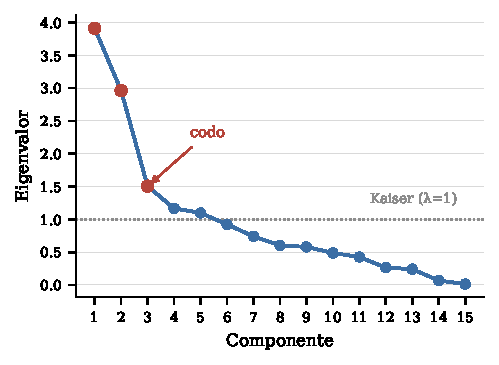
\includegraphics[width=0.92\linewidth]{pca_scree.pdf}

      \footnotesize Varianza explicada por componente.
    \end{column}
  \end{columns}
\end{frame}

% -----------------------------------------------------------------------
% Diapositiva 2: regresion logistica
% Fuente: reports/secciones/regresion_logistica.tex, subseccion
% "Regresion Logistica" y "Evaluacion y validacion del modelo".
% -----------------------------------------------------------------------
\begin{frame}{Regresión logística}
  \footnotesize

  \begin{block}{Partición y especificación}
    Entrenamiento 2021--2024, validación 2025. Predictores:
    \texttt{PC1}--\texttt{PC3} del ACP más 12 indicadoras
    (\texttt{zona}, \texttt{tipo\_dia}, \texttt{temporada}).
  \end{block}
  \vspace{-6pt}

  \begin{columns}[T]
    \begin{column}{0.56\textwidth}
      \textbf{Razones de momios por componente} (interpretadas por DE)
      \begin{itemize}[itemsep=1pt,topsep=2pt,parsep=0pt,leftmargin=*]
        \item \texttt{PC1} carga primaria: \textbf{1.47}
        \item \texttt{PC2} forzamiento fotoquímico: \textbf{1.58}
        \item \texttt{PC3} estancamiento: \textbf{1.22}
      \end{itemize}
      \textbf{Evaluación en validación} (umbral de Youden $=0.288$)
      \begin{itemize}[itemsep=1pt,topsep=2pt,parsep=0pt,leftmargin=*]
        \item AUC $=\mathbf{0.893}$ ($\geq 0.75$)
        \item Sensibilidad $=0.831$, especificidad $=0.824$
        \item Exactitud no se usa como criterio: tasa base de
          validación $=$ \textbf{41.50\,\%}
      \end{itemize}
    \end{column}
    \begin{column}{0.44\textwidth}
      \centering
      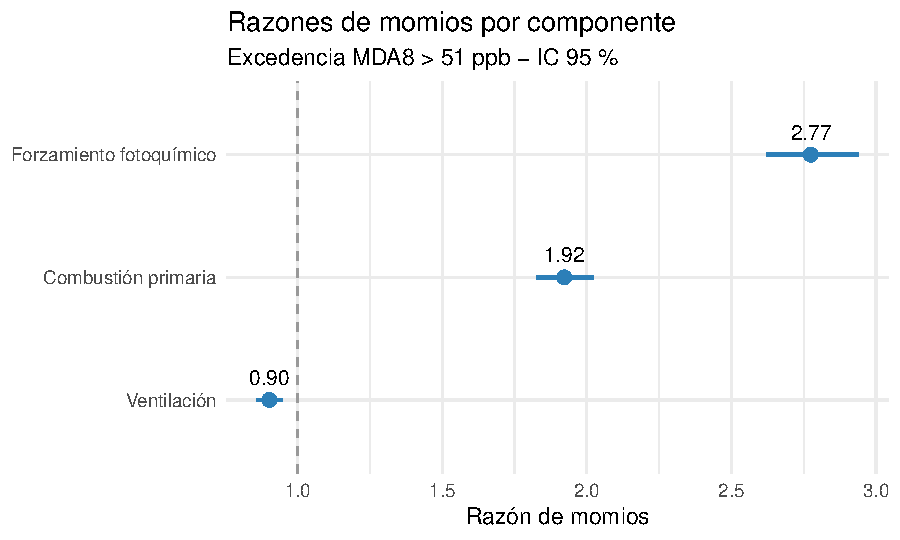
\includegraphics[width=\linewidth]{momios_componentes.pdf}
    \end{column}
  \end{columns}
\end{frame}

% -----------------------------------------------------------------------
% Diapositiva 3: discriminante + comparacion + cierre
% Fuente: reports/secciones/regresion_logistica.tex, subsecciones
% "Analisis discriminante lineal", "Comparacion de los dos modelos" y
% "Limitaciones".
% -----------------------------------------------------------------------
\begin{frame}{Discriminante lineal y comparación de modelos}
  \footnotesize

  \begin{columns}[T]
    \begin{column}{0.56\textwidth}
      \textbf{Supuestos del LDA}
      \begin{itemize}[itemsep=1pt,topsep=1pt,parsep=0pt,leftmargin=*]
        \item Normalidad: sesgos Box--Cox $<0.5$; se sostiene
        \item Homocedasticidad: \textbf{no se cumple} (razones de DE
          0.88/0.69/0.92 por componente; varianza generalizada
          $19.6 \to 6.1$)
      \end{itemize}
      \textbf{Resultado} (validación, Youden $=0.293$)
      \begin{itemize}[itemsep=1pt,topsep=1pt,parsep=0pt,leftmargin=*]
        \item AUC $=\mathbf{0.893}$; sensibilidad $0.845$;
          especificidad $0.811$
      \end{itemize}
      \textbf{Comparación con la logística}
      \begin{itemize}[itemsep=1pt,topsep=1pt,parsep=0pt,leftmargin=*]
        \item AUC coincide a 4 decimales (0.8928 ambos); DeLong
          $Z=0.011$, $p=0.99$
        \item Clasificaciones coinciden en el \textbf{98.1\,\%} de los
          días
      \end{itemize}
    \end{column}
    \begin{column}{0.44\textwidth}
      \centering
      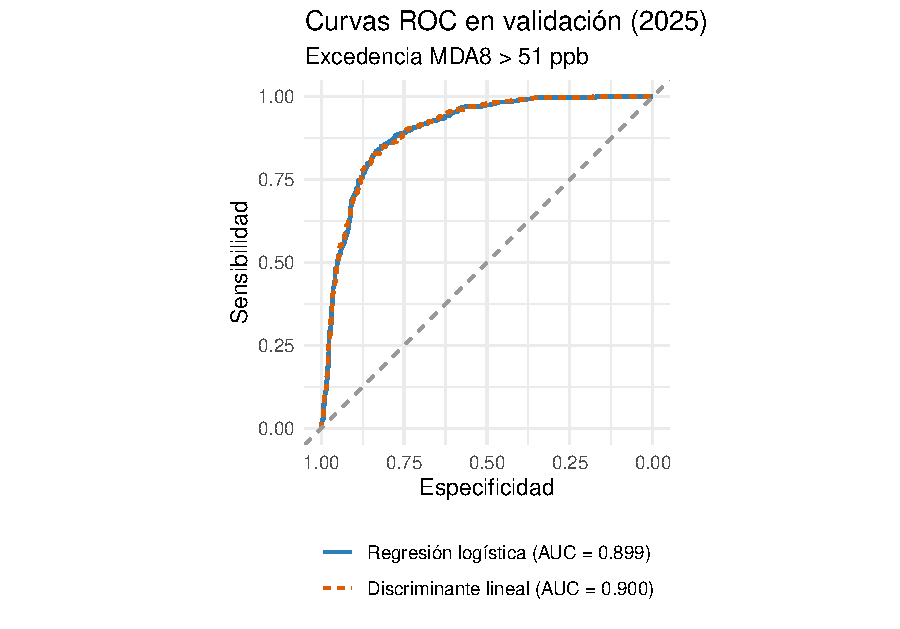
\includegraphics[width=\linewidth]{roc_modelos.pdf}
    \end{column}
  \end{columns}
  \vspace{3pt}

  \textbf{Cierre.} La heterocedasticidad documentada es real y no
  altera el desempeño: la frontera de decisión es prácticamente la
  misma con o sin ese supuesto. Limitaciones: autocorrelación
  espacio-temporal (muestra efectiva $\approx 1\,642$ días, no
  17{,}002 filas), sin datos de COV, y alcance estrictamente
  explicativo (mismo día, no predictivo).
\end{frame}

\end{document}
